%%%%%%%%%%%%%%%%%%%%%%%%%%%%%%%%%%%%%%%%%%%%%%%%%%%%%%%%%%%%%%%%%%%%%
% LaTeX Template: Softwaretechnik SS 2017
%
% Date: April 2017
%
%%%%%%%%%%%%%%%%%%%%%%%%%%%%%%%%%%%%%%%%%%%%%%%%%%%%%%%%%%%%%%%%%%%%%%

\documentclass[12pt]{article}
\usepackage[a4paper]{geometry}
\usepackage{framed}
\usepackage[myheadings]{fullpage}
\usepackage{fancyhdr}
\usepackage{lastpage}
\usepackage{graphicx, wrapfig, subcaption, setspace, booktabs}


\usepackage[font=small, labelfont=bf]{caption}
\usepackage[protrusion=true, expansion=true]{microtype}
\usepackage[ngerman]{babel}
\usepackage[ngerman]{translator}
\usepackage{sectsty}
\usepackage{url, lipsum}
\usepackage[parfill]{parskip}
\usepackage{csquotes}
\usepackage[hidelinks]{hyperref}
\usepackage[acronym]{glossaries}

\usepackage[sorting=none,backref=true, backend=biber]{biblatex}
\addbibresource{\jobname.bib}
\usepackage[export]{adjustbox}
\usepackage{multicol}
\usepackage{tikz}
\usepackage{float}
\usepackage{pdfpages}
% \usepackage{xcolor}


\makeglossaries
\glstoctrue

\usepackage{listings}
\usepackage{color}

\usepackage{dirtree}
\input dirtree

\definecolor{dkgreen}{rgb}{0,0.6,0}
\definecolor{gray}{rgb}{0.5,0.5,0.5}
\definecolor{mauve}{rgb}{0.58,0,0.82}
\definecolor{dandelion}{HTML}{FDBC42}

\lstset{
  % frame=tblr,
  language=Java,
  aboveskip=3mm,
  belowskip=3mm,
  showstringspaces=false,
  columns=flexible,
  basicstyle={\small\ttfamily},
  % numbers=left,
  numberstyle=\tiny\color{gray},
  keywordstyle=\color{blue},
  commentstyle=\color{dkgreen},
  % morecomment=[s][\color{orange}]{@}{\ },
  stringstyle=\color{mauve},
  breaklines=true,
  breakatwhitespace=true,
  tabsize=3,
  moredelim=[is][\textcolor{orange}]{\~\~}{\~\~},
  moredelim=[il][\textcolor{dandelion}]{\$\$},
  moredelim=[is][\textcolor{dandelion}]{\%\%}{\%\%}
}

\DTsetlength{ 0.2em}{ 1em}{ 0.2em}{ 0.4pt}{ 0.1pt}

\usepackage[T1]{fontenc}
%-------------------------------------------------------------------------------
% Commands
%-------------------------------------------------------------------------------
\newcommand{\HRule}[1]{\rule{\linewidth}{#1}}
\input{../env}
%-------------------------------------------------------------------------------
% HEADER & FOOTER
%-------------------------------------------------------------------------------
\fancypagestyle{myplain}
{
\fancyhf{}
\paperwidth=\pdfpageheight
\paperheight=\pdfpagewidth
\pdfpageheight=\paperheight
\pdfpagewidth=\paperwidth
\headwidth=\textwidth
\renewcommand\headrulewidth{0pt}
\renewcommand\footrulewidth{0pt}
\fancyfoot[R]{Seite \thepage\ von \pageref{LastPage}}

}

\fancypagestyle{myfancy}{
  \fancyhf{}
  \pagestyle{fancy}
  \fancyhf{}
  \setlength\headheight{15pt}
  \fancyhead[L]{\newCommandName}
  \fancyhead[R]{\newCommandUniversity}
  \fancyfoot[R]{Seite \thepage\ von \pageref{LastPage}}
}

%-------------------------------------------------------------------------------
% TITLE PAGE
%-------------------------------------------------------------------------------
\begin{document}
\hypersetup{
    % colorlinks,
    citecolor=black,
    filecolor=black,
    linkcolor=black,
    urlcolor=black
}


\title{ \normalsize
		\HRule{0.5pt} \\
		\LARGE \textbf{\uppercase{\newCommandDiscipline}} \\
    \smallbreak
    \small\textbf{{SVN - Versions- und Fehlermanagement}}\\
		\HRule{2pt} \\ [0.5cm]
    \small\textbf{{\newCommandTerm}}\\
    [0.5cm]
    \normalsize \today \vspace*{10\baselineskip}}

\date{}



\author{
    \newCommandName \\
		\newCommandMatriculationNumber \\
		\newCommandUniversity \\
		\newCommandFaculty
}

% \pagenumbering{gobble}

\maketitle
\thispagestyle{empty}

\newpage
\pagestyle{myfancy}
\tableofcontents
% \listoffigures
\newpage

%-------------------------------------------------------------------------------
% Section title formatting
\sectionfont{\scshape}
%-------------------------------------------------------------------------------

%-------------------------------------------------------------------------------
% BODY
%-------------------------------------------------------------------------------
\section{SVN - Versions- und Fehlermanagement}

\subsection{Pull Request}

\textbf{Screenshot vom Pull-Request:}

\begin{figure}[H]
  \centering
  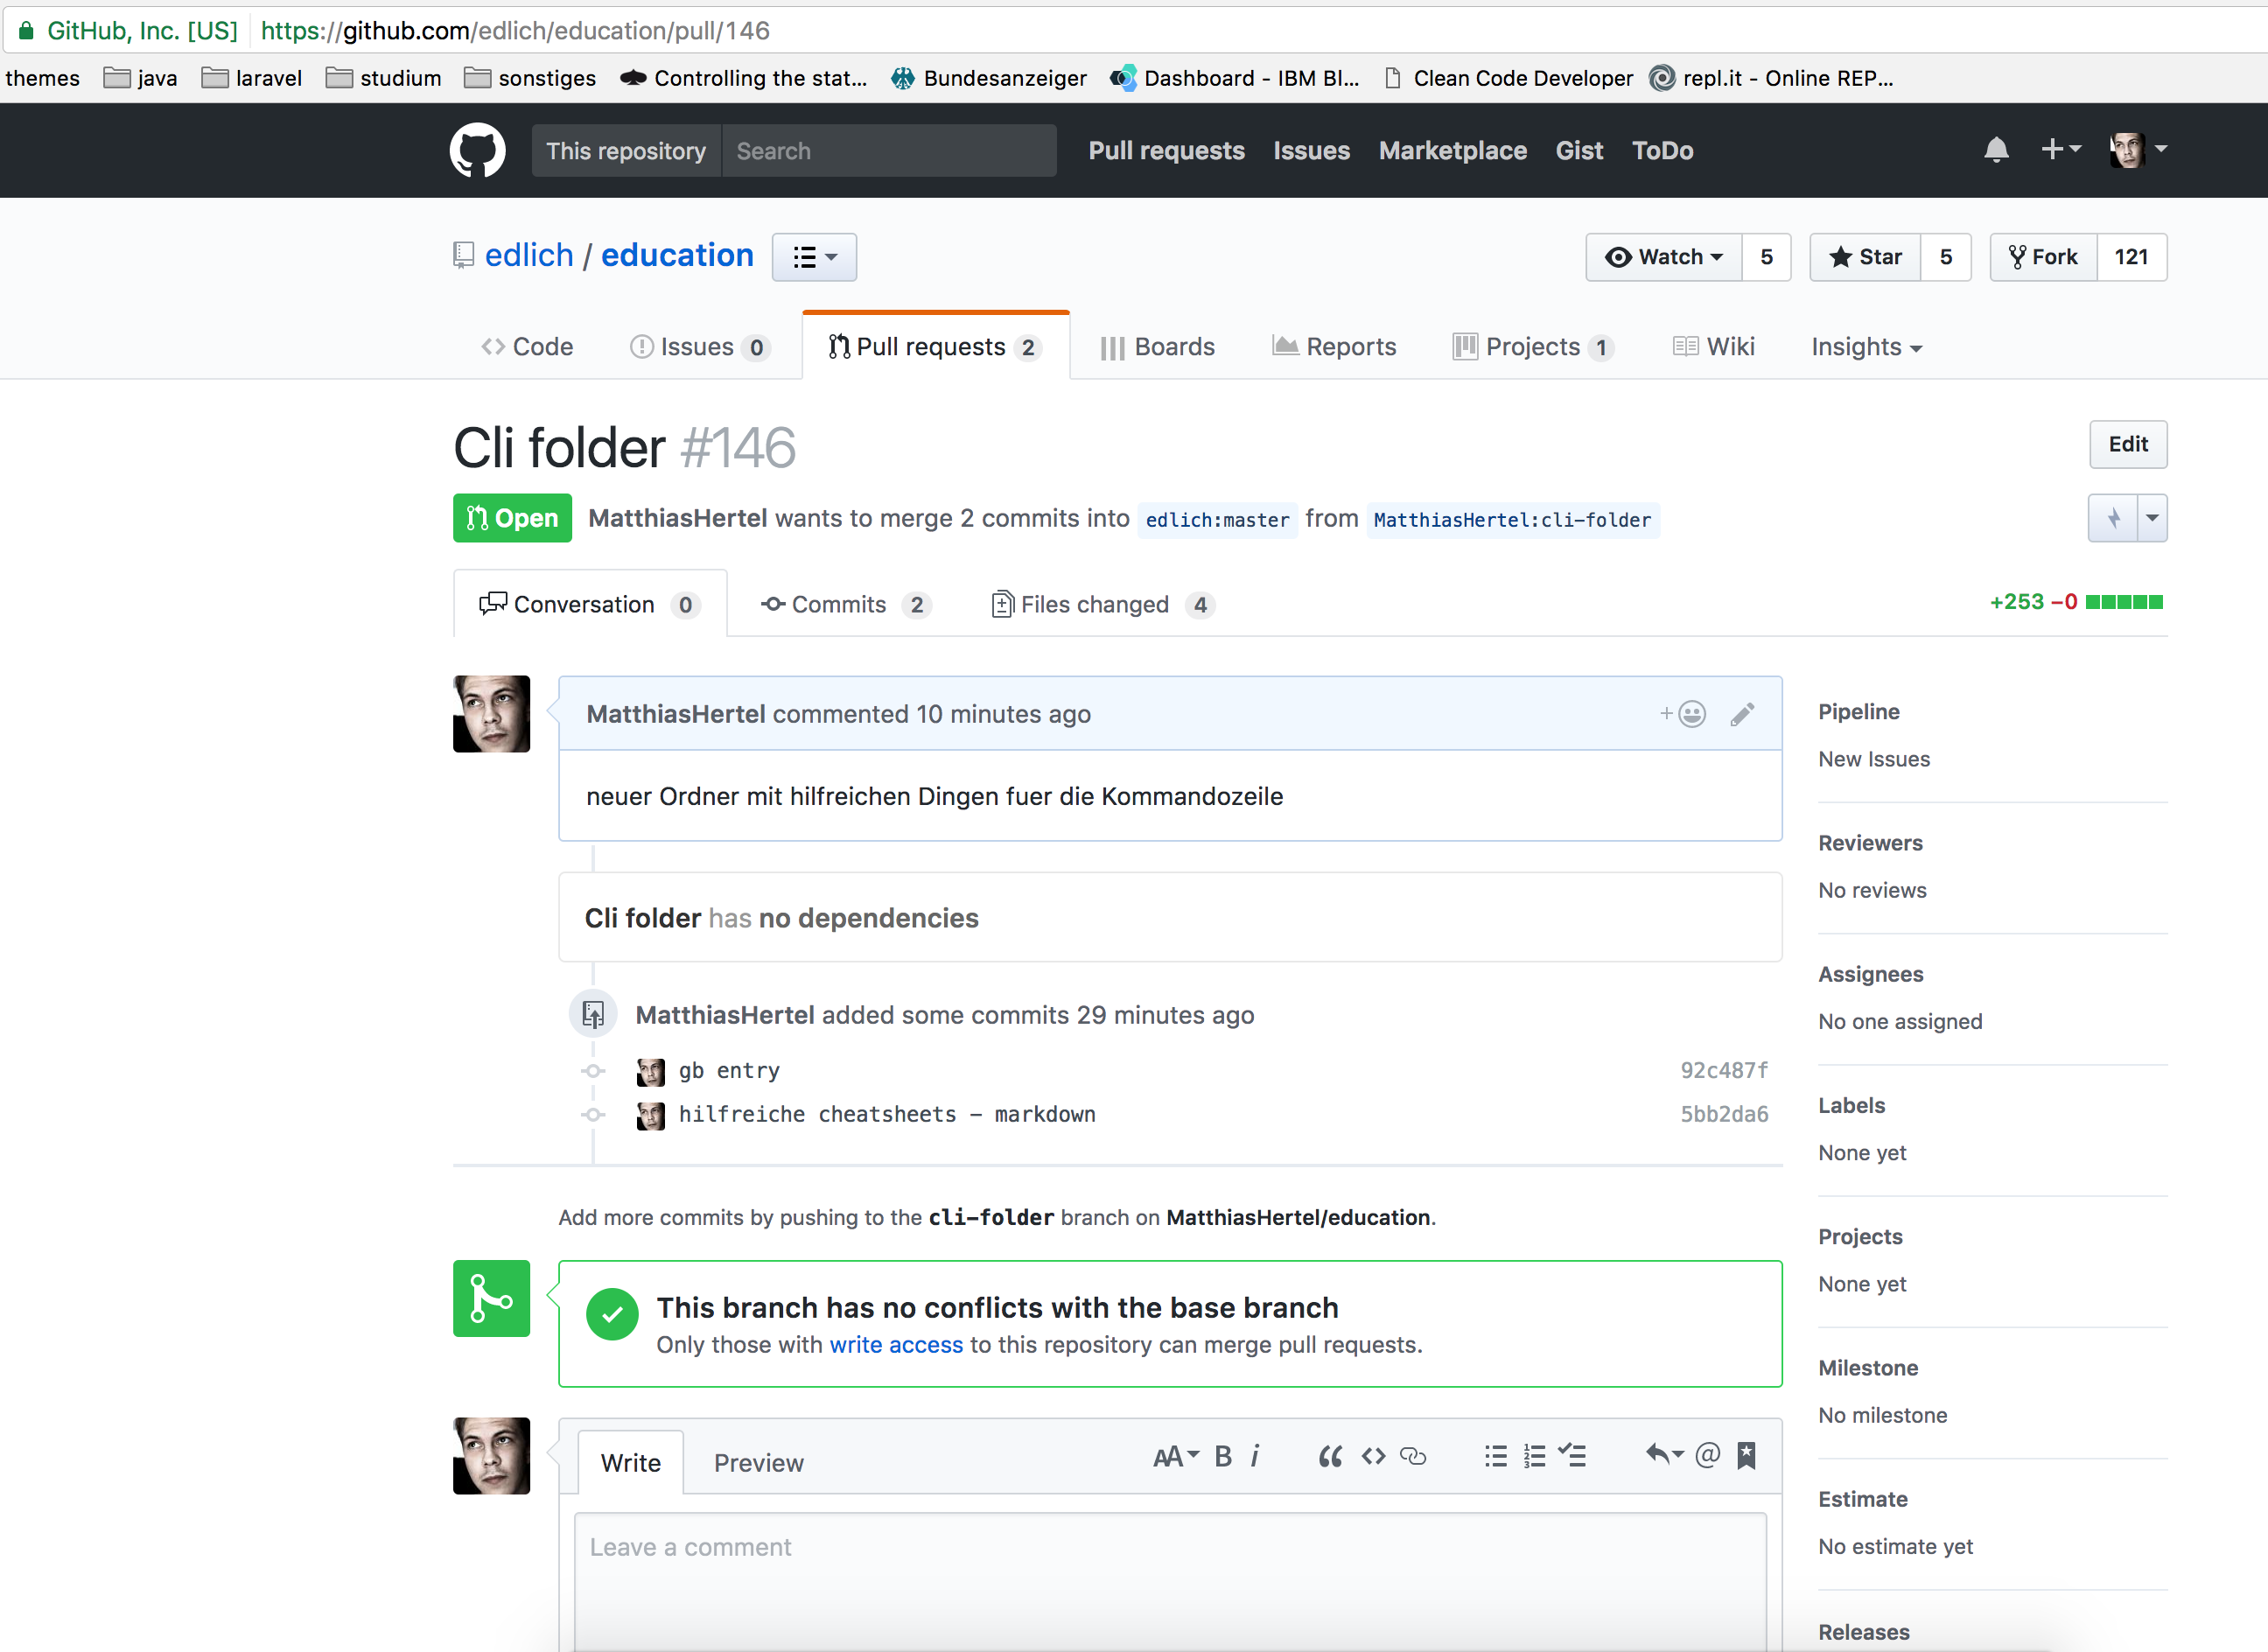
\includegraphics[width=0.9\textwidth]{./img/pull_request.png}
  \captionsetup{name=Abb.,font=footnotesize}
  \caption{Screenshot vom Pull-Request (CLI-Folder)}
\end{figure}

\newpage
\subsection{Beispiel Repos}
\subsubsection{Git Repo Softwaretechnik - Einsendeaufgaben in Tex}

\textbf{SSH:}

git clone git@github.com:MatthiasHertel/softwaretechnik.git


\textbf{Download:}

https://github.com/MatthiasHertel/softwaretechnik/archive/master.zip

\subsubsection{Git Repo Softwaretechnik - eigenes Softwareprojekt}

\textbf{SSH:}

git clone git@github.com:MatthiasHertel/productstore.git


\textbf{Download:}

https://github.com/MatthiasHertel/productstore/archive/master.zip


\newpage
\subsection{Beispiel Screenshots von der Arbeit mit GIT}

\subsubsection{git status  git add}

\begin{figure}[H]
  \centering
  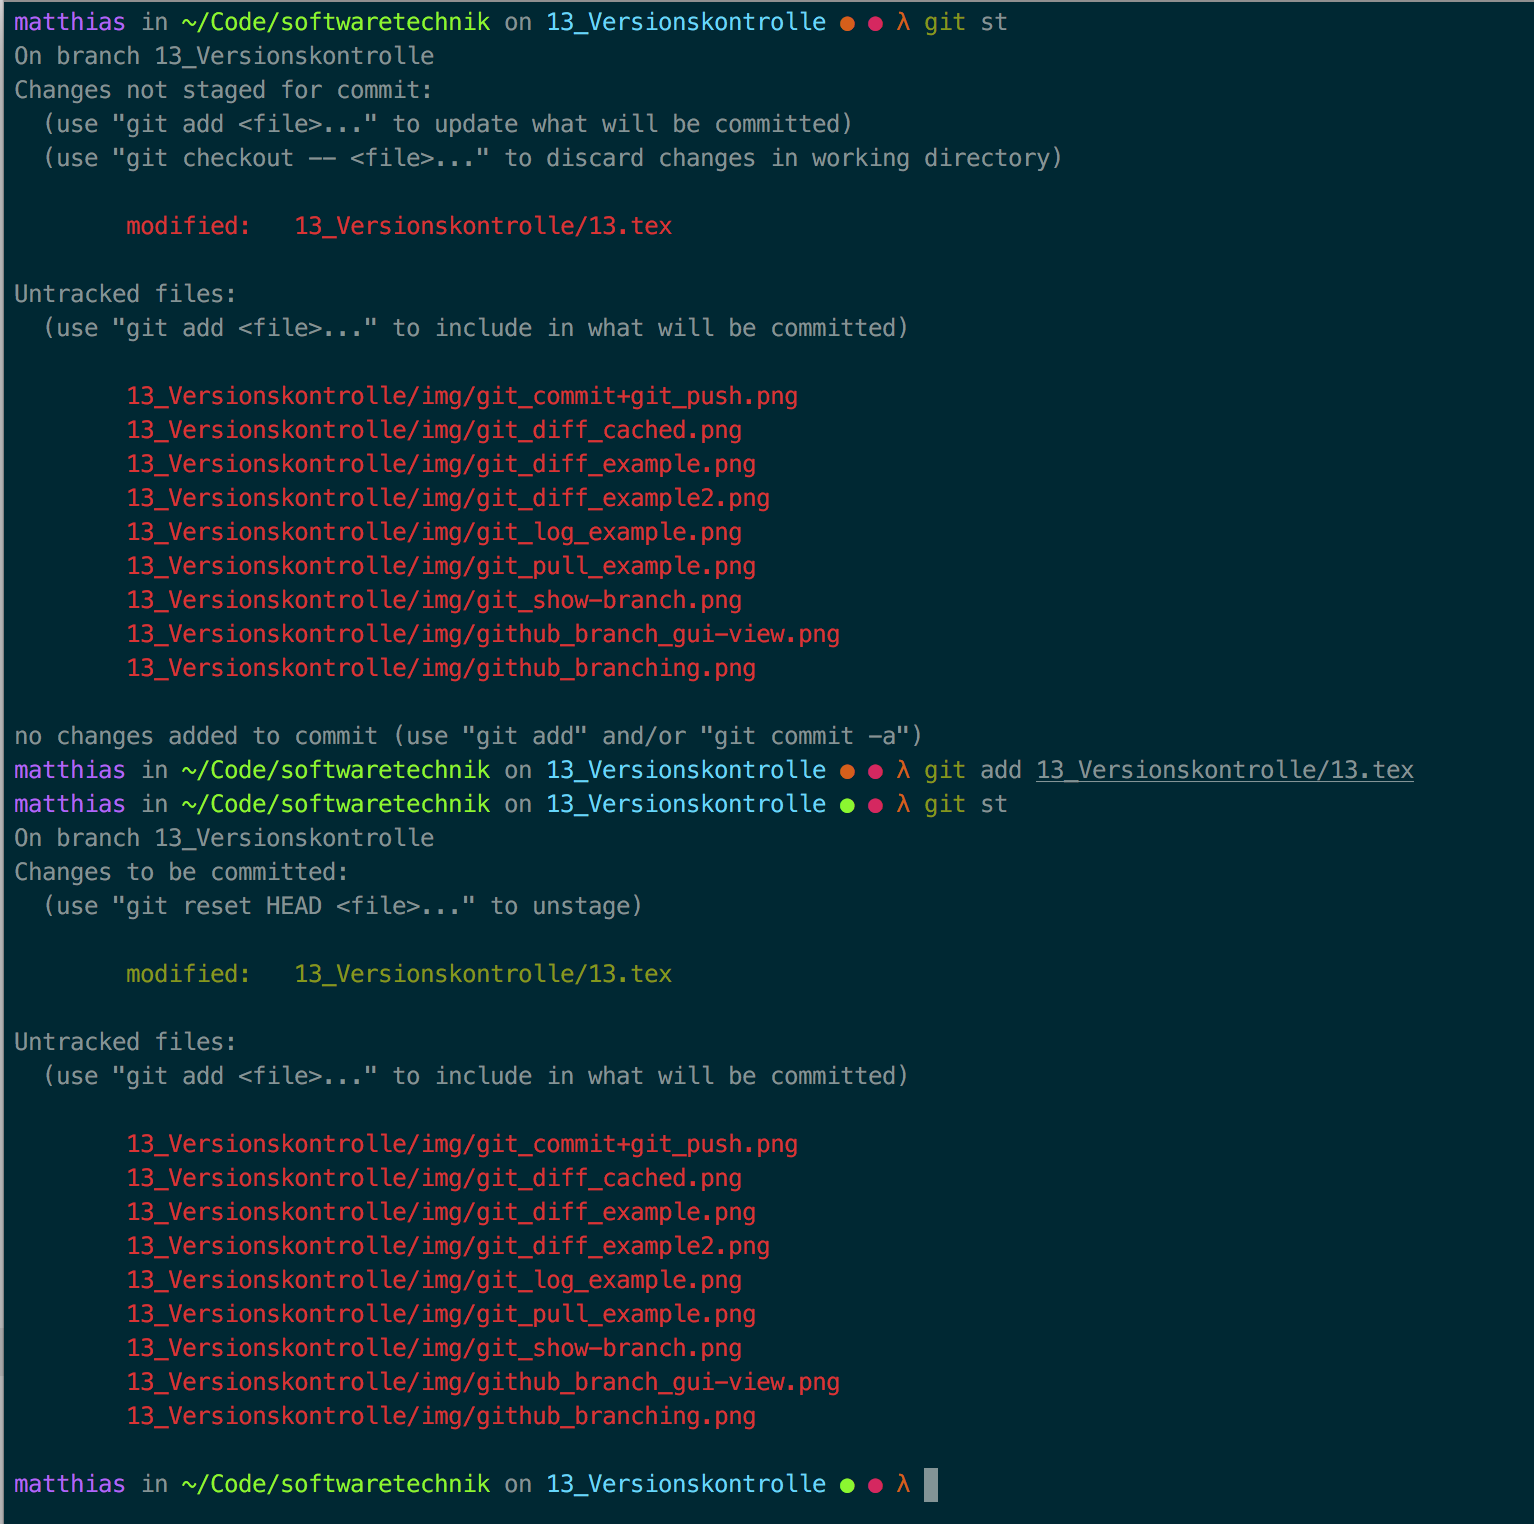
\includegraphics[width=0.7\textwidth]{./img/git_status_git_add.png}
  \captionsetup{name=Abb.,font=footnotesize}
  \caption{Status und Files f"ur Commit vorbereiten.}
\end{figure}

\subsubsection{git diff}

\begin{figure}[H]
  \centering
  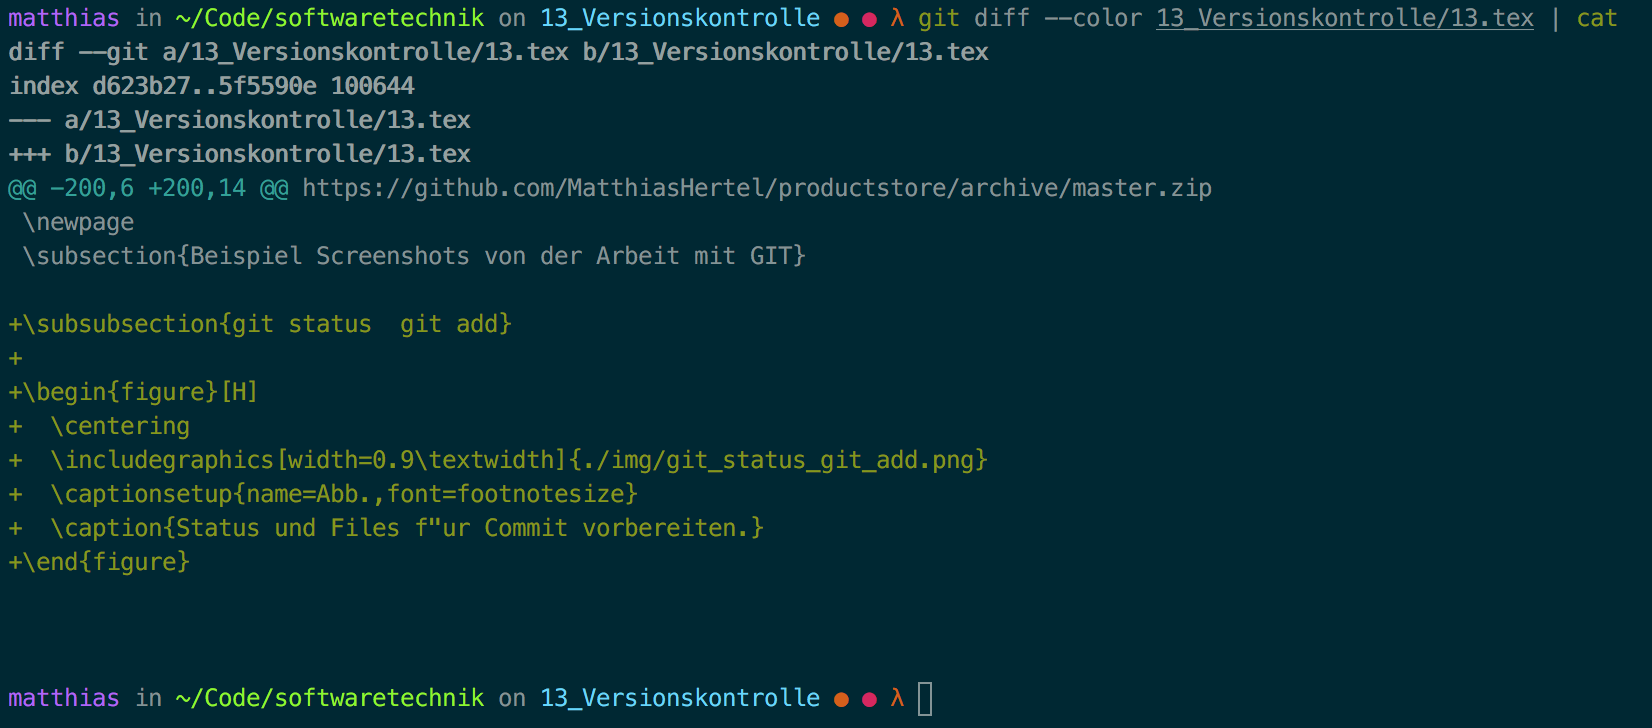
\includegraphics[width=0.7\textwidth]{./img/git_diff.png}
  \captionsetup{name=Abb.,font=footnotesize}
  \caption{git diff - zeigt unterschiede zwischen commits}
\end{figure}

\subsubsection{git commit git push}
\subsubsection{furthermore git branching}




%-------------------------------------------------------------------------------
% Literatur - Glossar - Akronyme
%-------------------------------------------------------------------------------

% \clearpage
% \setlength\bibitemsep{10pt}
% \printbibliography[heading=bibintoc]
% \newpage
% \printglossary[type=main,title=Glossar]
% \printglossary[type=\acronymtype, title=Akronyme]


%-------------------------------------------------------------------------------
% ENDE
%-------------------------------------------------------------------------------

\end{document}
